This Appendix shows the event yields and distributions of \mjj prior 
to the fit to data (Table~\ref{tab:eventYieldAppend} and 
Fig.~\ref{fig:mjjPreFit}) and the upper limits on $\mathcal{B}(\PQt \to
\PSHp\PQb)$ from the individual charm tagging categories 
(Fig.~\ref{fig:limitAppend}).

\begin{table}[ht]
  \centering
  \topcaption{Expected event yields, prior to the fit, for backgrounds 
    in each of the channels and event categories. The number of events,
    along with the uncertainty prior to fit (including statistical and  
    systematic effects), is shown.}
  \label{tab:eventYieldAppend}
  \cmsTable{
\begin{tabular}{cccccccc}
\hline
\hline
\textbf{Process} & \multicolumn{2}{c}{Loose} & \multicolumn{2}{c}{Medium} & \multicolumn{2}{c}{Tight} \\
                  & $\mu$ + jets   &  e + jets      & $\mu$ + jets   &  e + jets      & $\mu$ + jets   &  e + jets \\
\hline
\hline
SM $\ttbar$ + jets & 100295 $\pm$ 9241 & 74479 $\pm$ 6853 & 76226 $\pm$ 7398 & 56556 $\pm$ 5474 & 19728 $\pm$ 2321 & 14528 $\pm$ 1643\\
Single \PQt & 2861 $\pm$ 327 & 2159 $\pm$ 262 & 2126 $\pm$ 250 & 1585 $\pm$ 191 & 483 $\pm$ 66 & 355 $\pm$ 49\\
QCD multijet & 1772 $\pm$ 140 & 1402 $\pm$ 108 & 1067 $\pm$ 124 & 1077 $\pm$ 109 & 202 $\pm$ 56 & 296 $\pm$ 54\\
\PW + jets & 1609 $\pm$ 384 & 1181 $\pm$ 199 & 1131 $\pm$ 270 & 792 $\pm$ 144 & 144 $\pm$ 47 & 110 $\pm$ 37\\
$\PZ/\PGg$ + jets & 198 $\pm$ 46 & 250 $\pm$ 53 & 143 $\pm$ 36 & 153 $\pm$ 34 & 61 $\pm$ 15 & 35 $\pm$ 9\\
VV & 70 $\pm$ 18 & 52 $\pm$ 16 & 68 $\pm$ 30 & 16 $\pm$ 10 & 14 $\pm$ 9 & 4 $\pm$ 4\\
\hline 
All background & 106805 $\pm$ 9936 & 79523 $\pm$ 7349 & 80761 $\pm$ 7918 & 60179 $\pm$ 5829 & 20632 $\pm$ 2422 & 15329 $\pm$ 1720\\
\hline 
Data & 105485 & 77244 & 76811 & 56051 & 19451 & 14179 \\
\hline 
\end{tabular}
}
\end{table}


\begin{figure}
\centering  
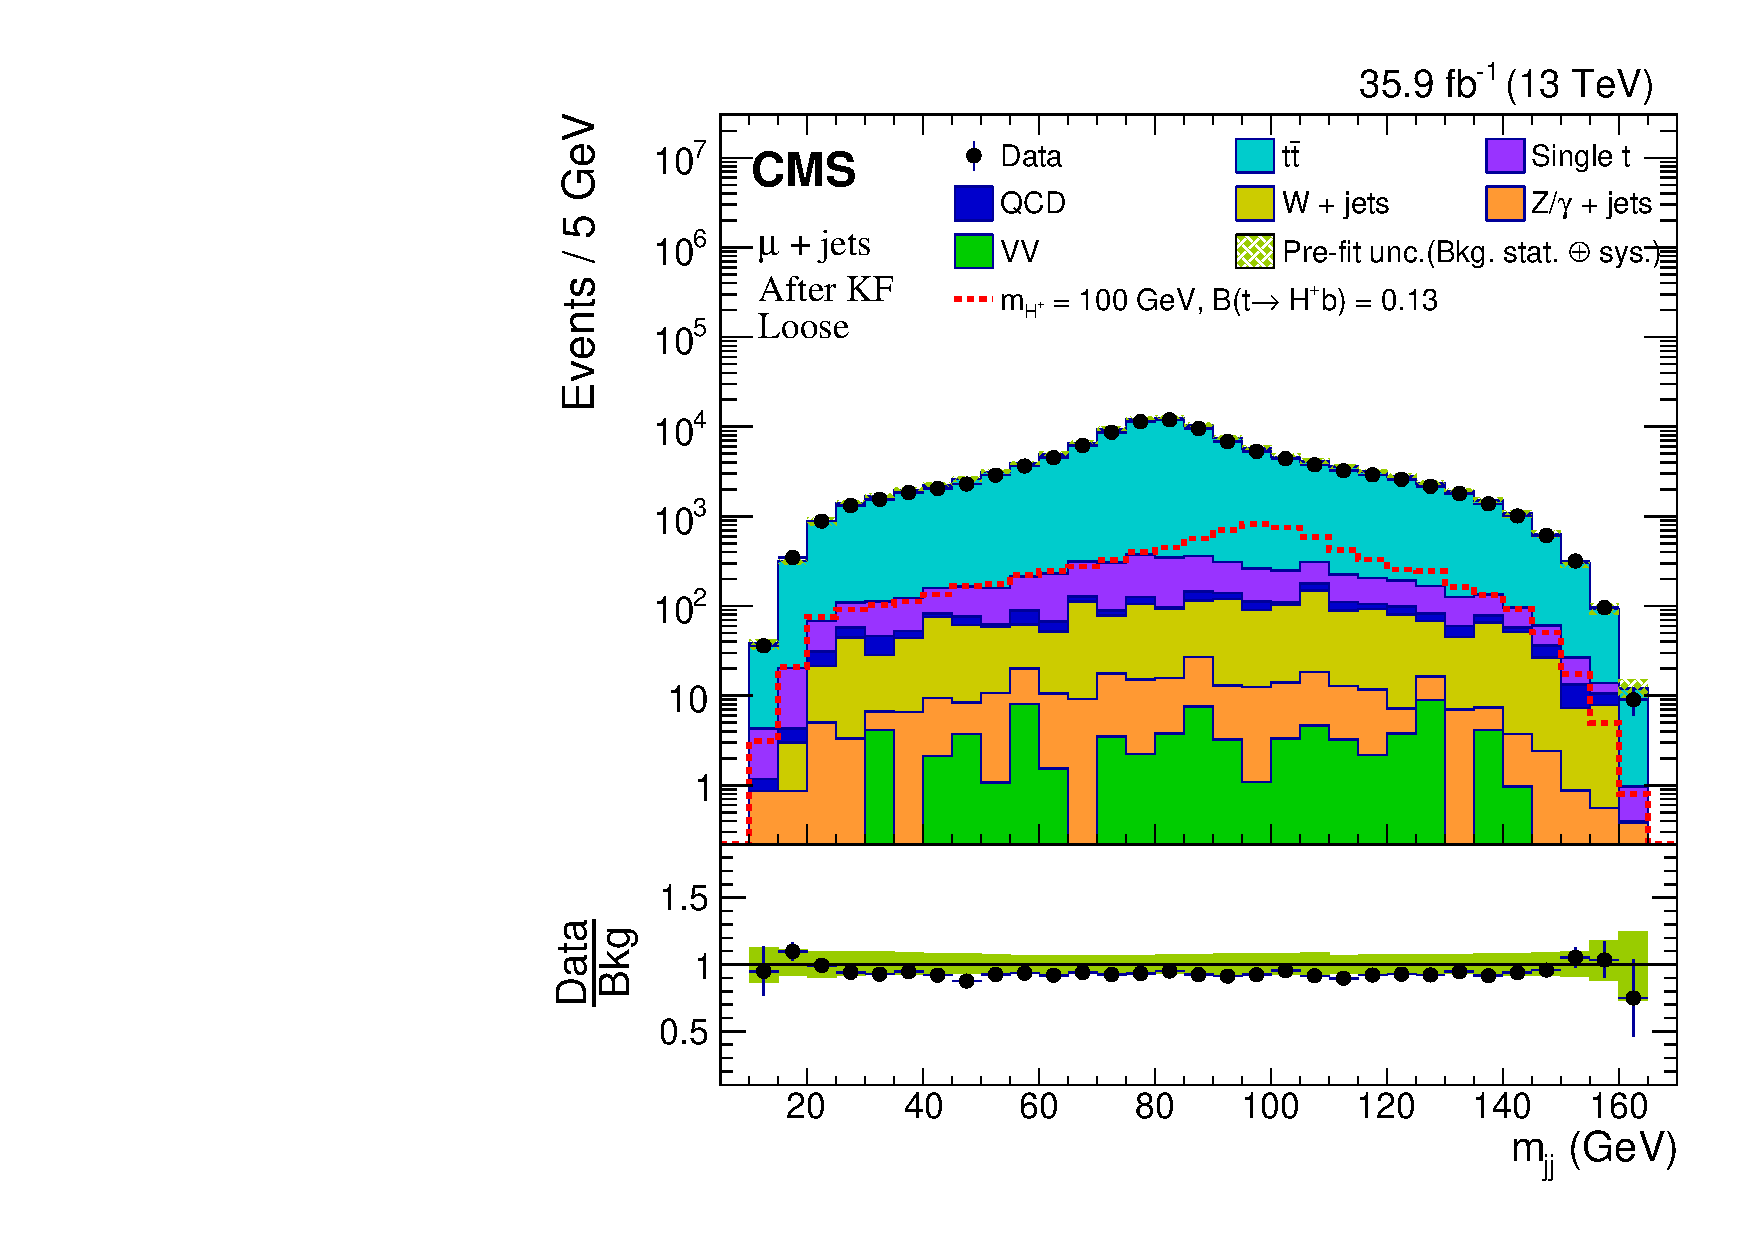
\includegraphics[width=0.44\textwidth]{Image/Appendix/mjj_kfit_CTagExL_muKinFit.pdf}
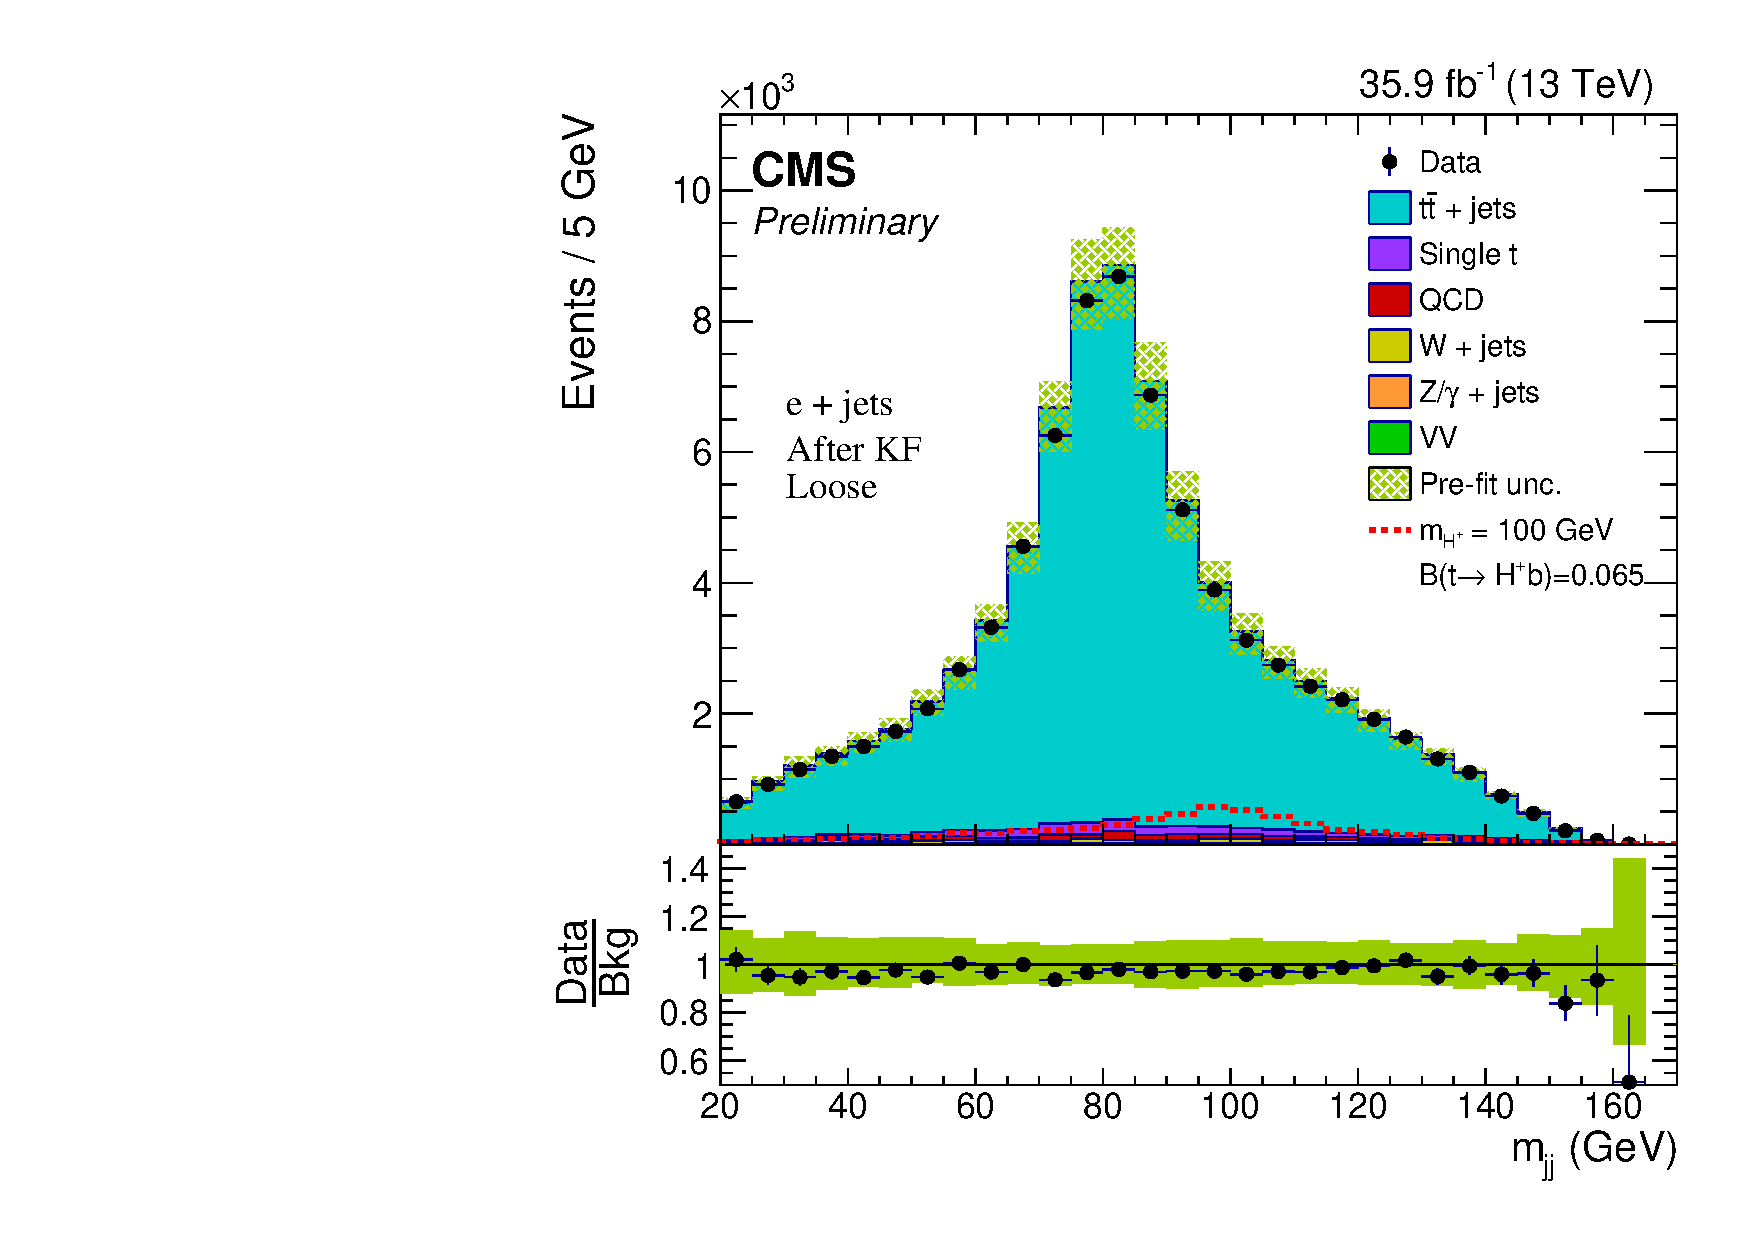
\includegraphics[width=0.44\textwidth]{Image/Appendix/mjj_kfit_CTagExL_eleKinFit.pdf}
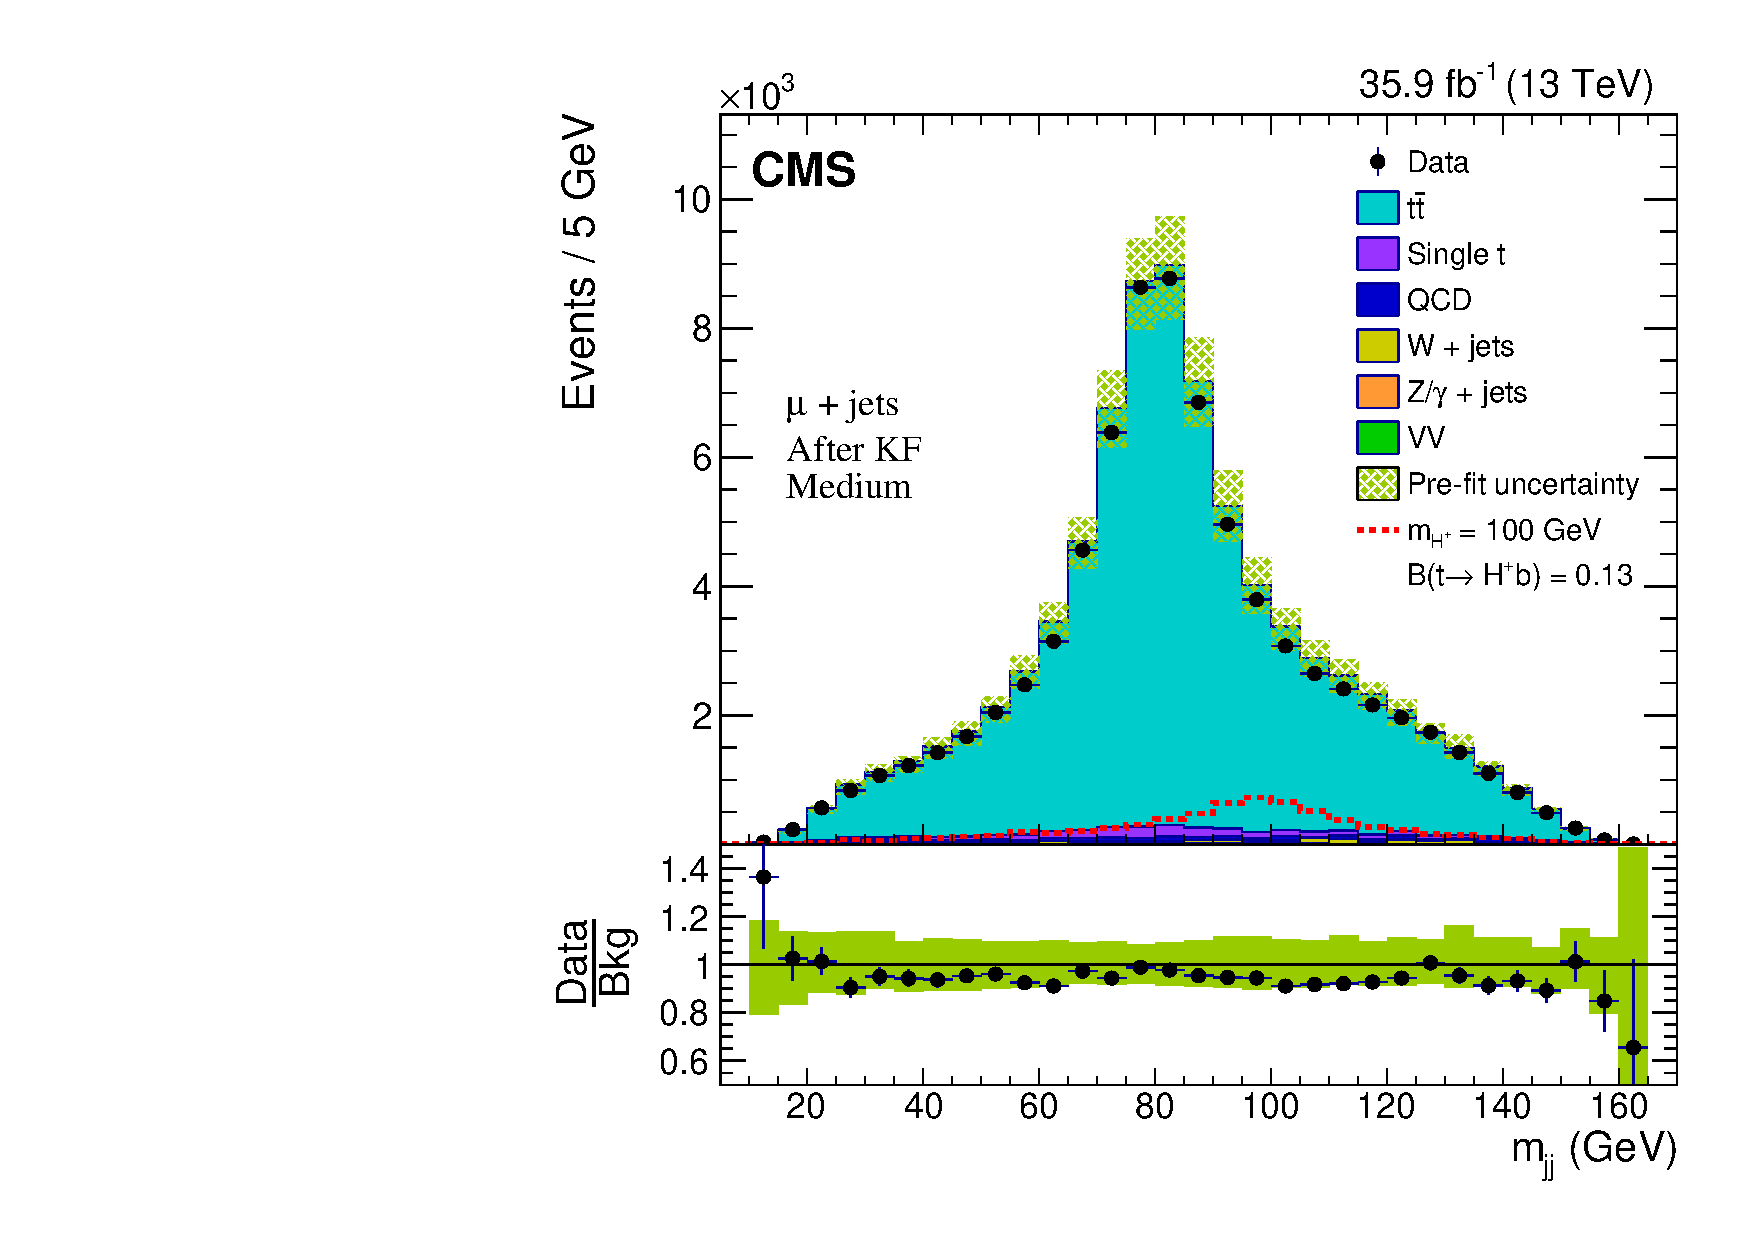
\includegraphics[width=0.44\textwidth]{Image/Appendix/mjj_kfit_CTagExM_muKinFit.pdf}
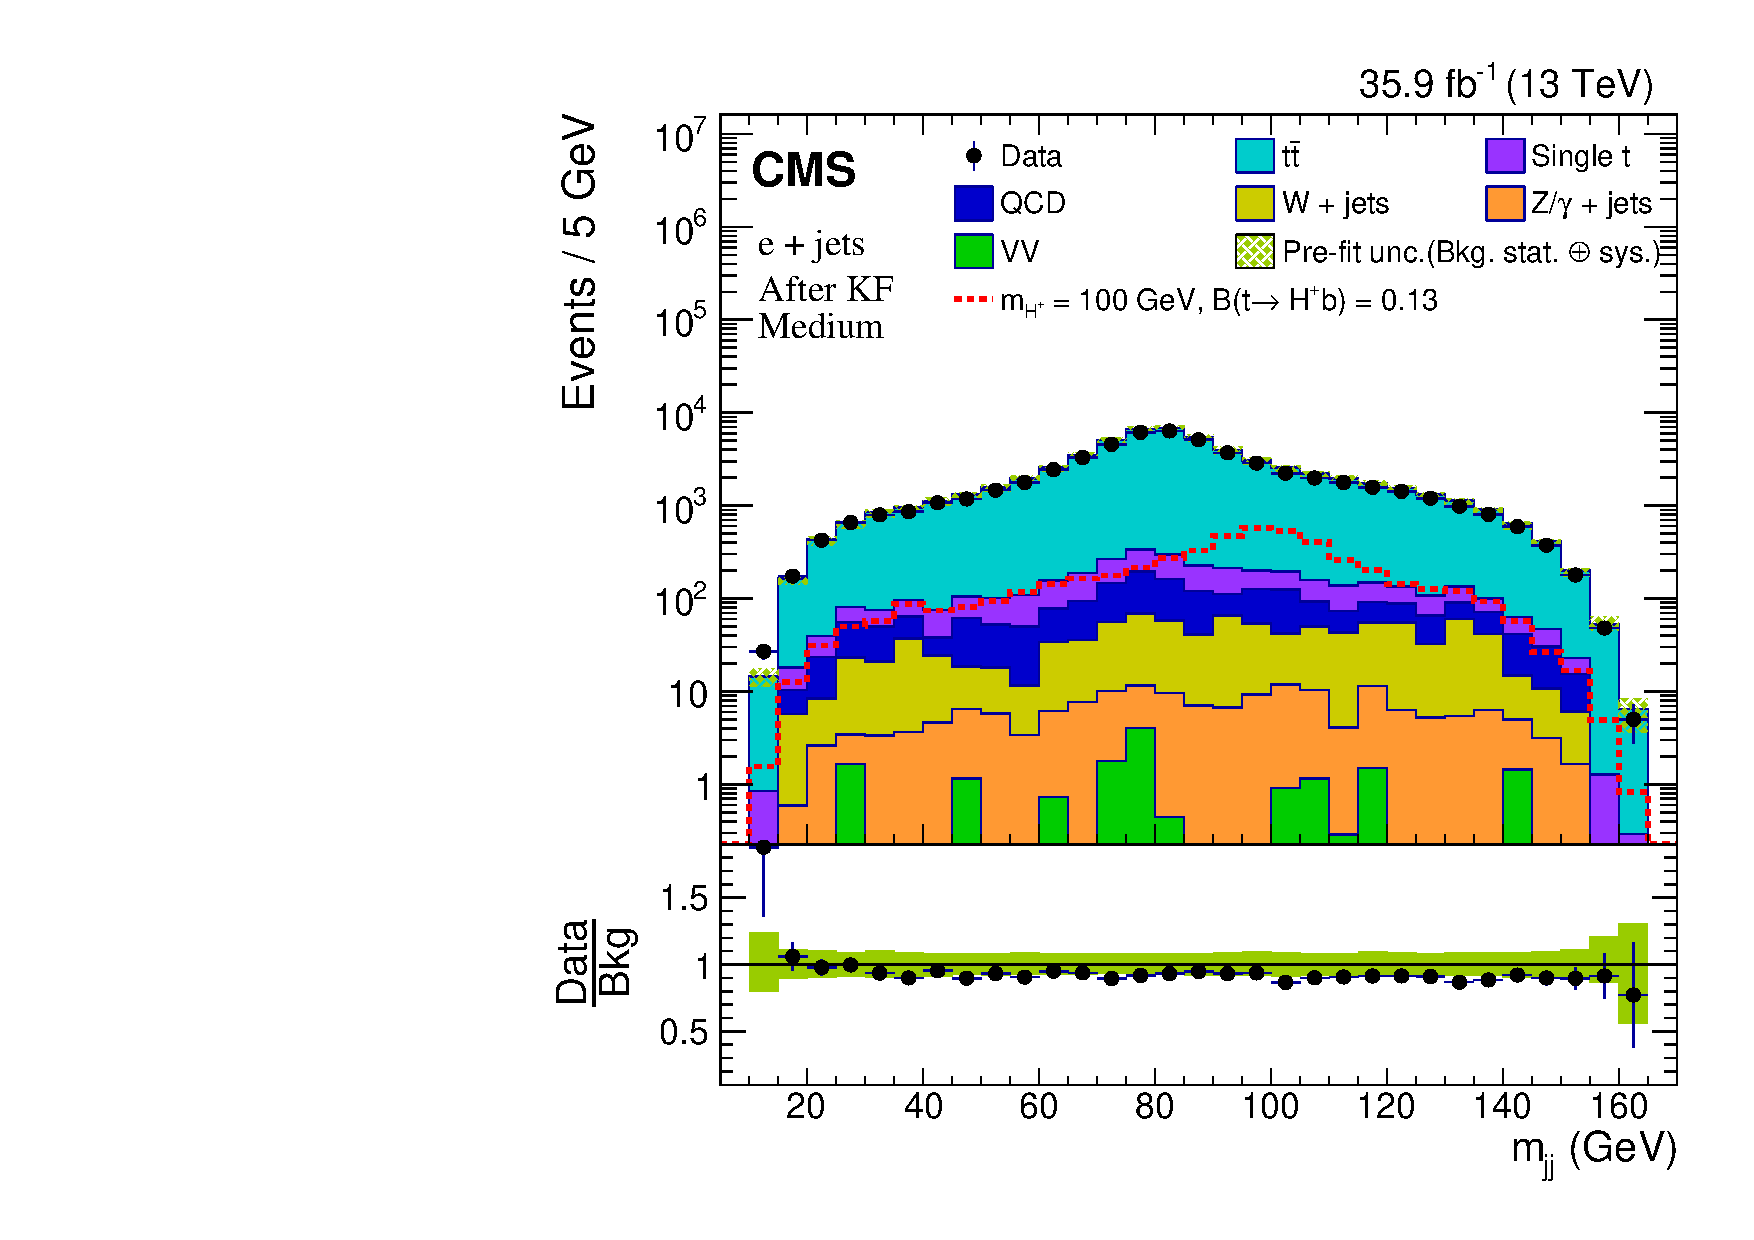
\includegraphics[width=0.44\textwidth]{Image/Appendix/mjj_kfit_CTagExM_eleKinFit.pdf}
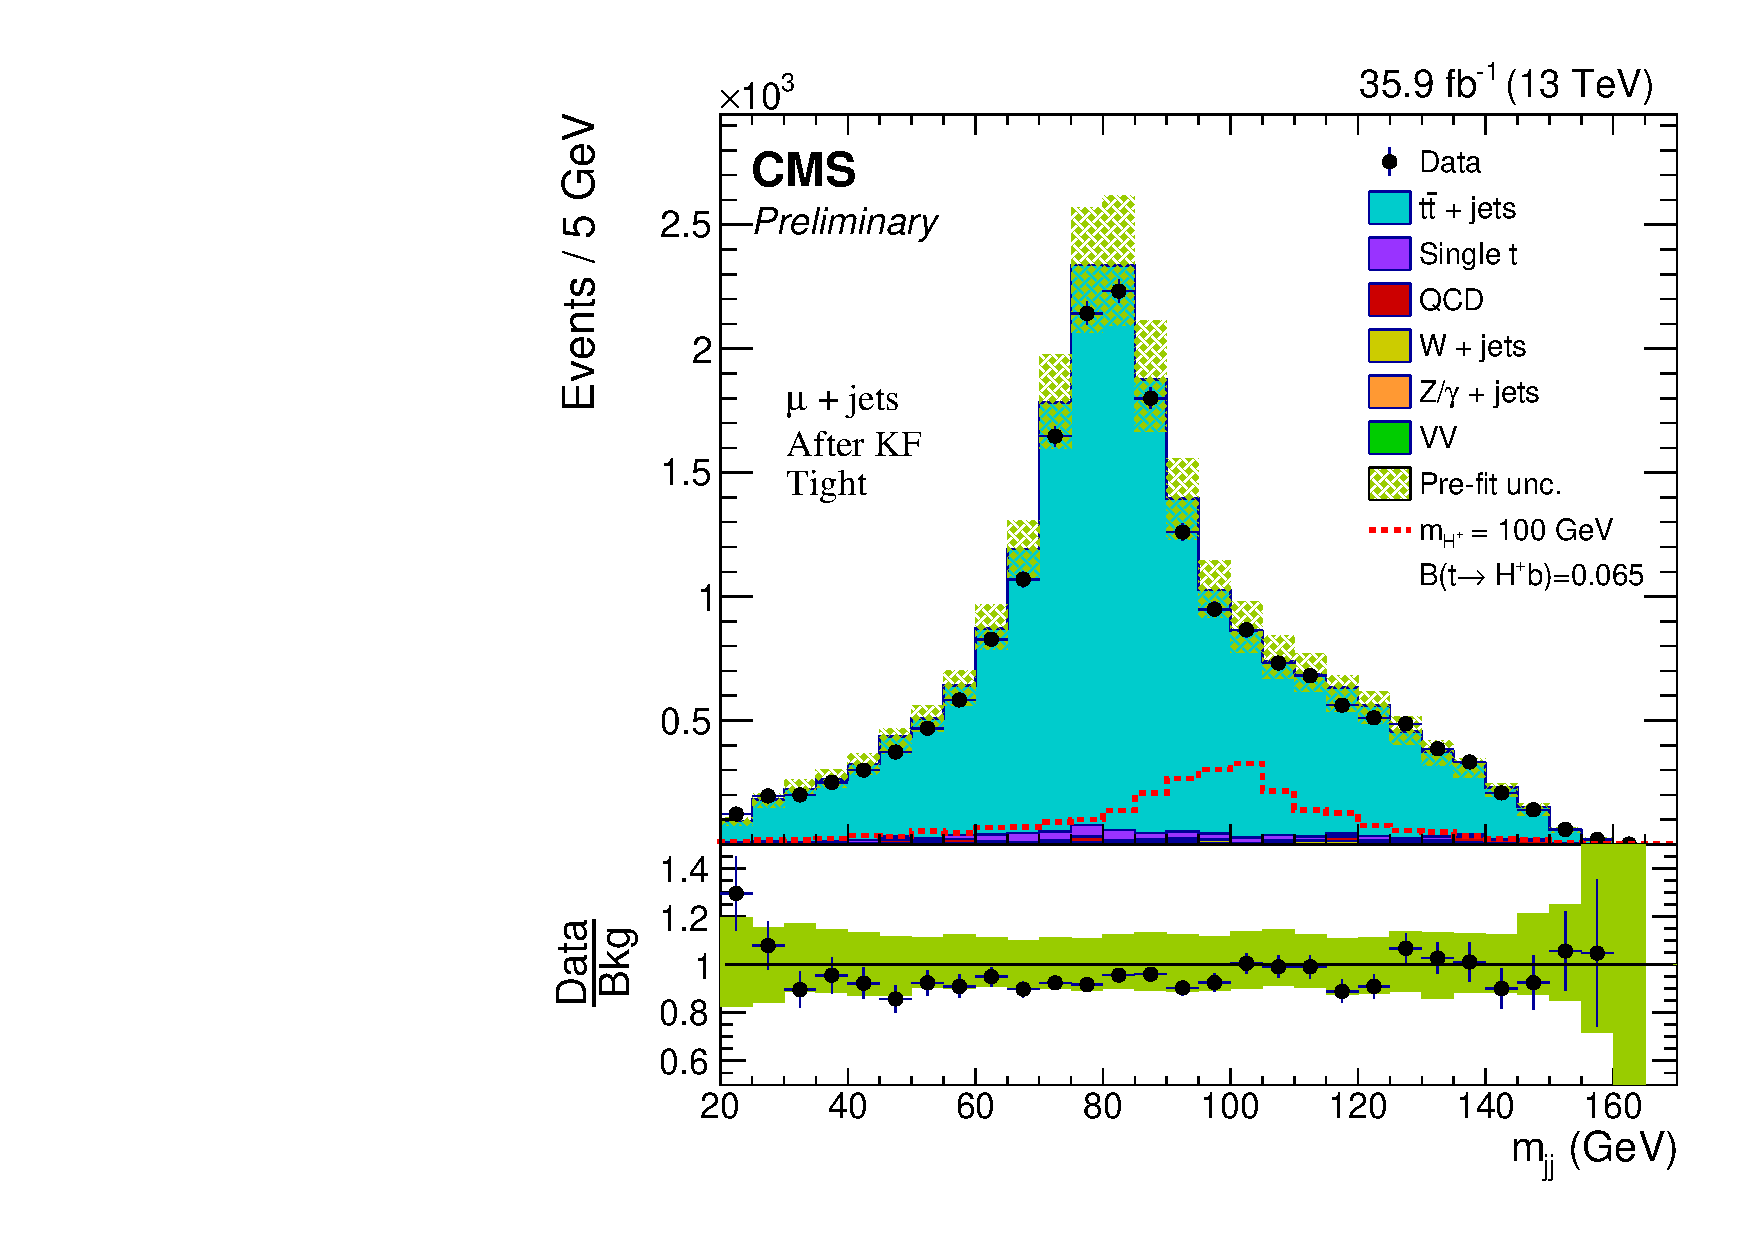
\includegraphics[width=0.44\textwidth]{Image/Appendix/mjj_kfit_CTagExT_muKinFit.pdf}
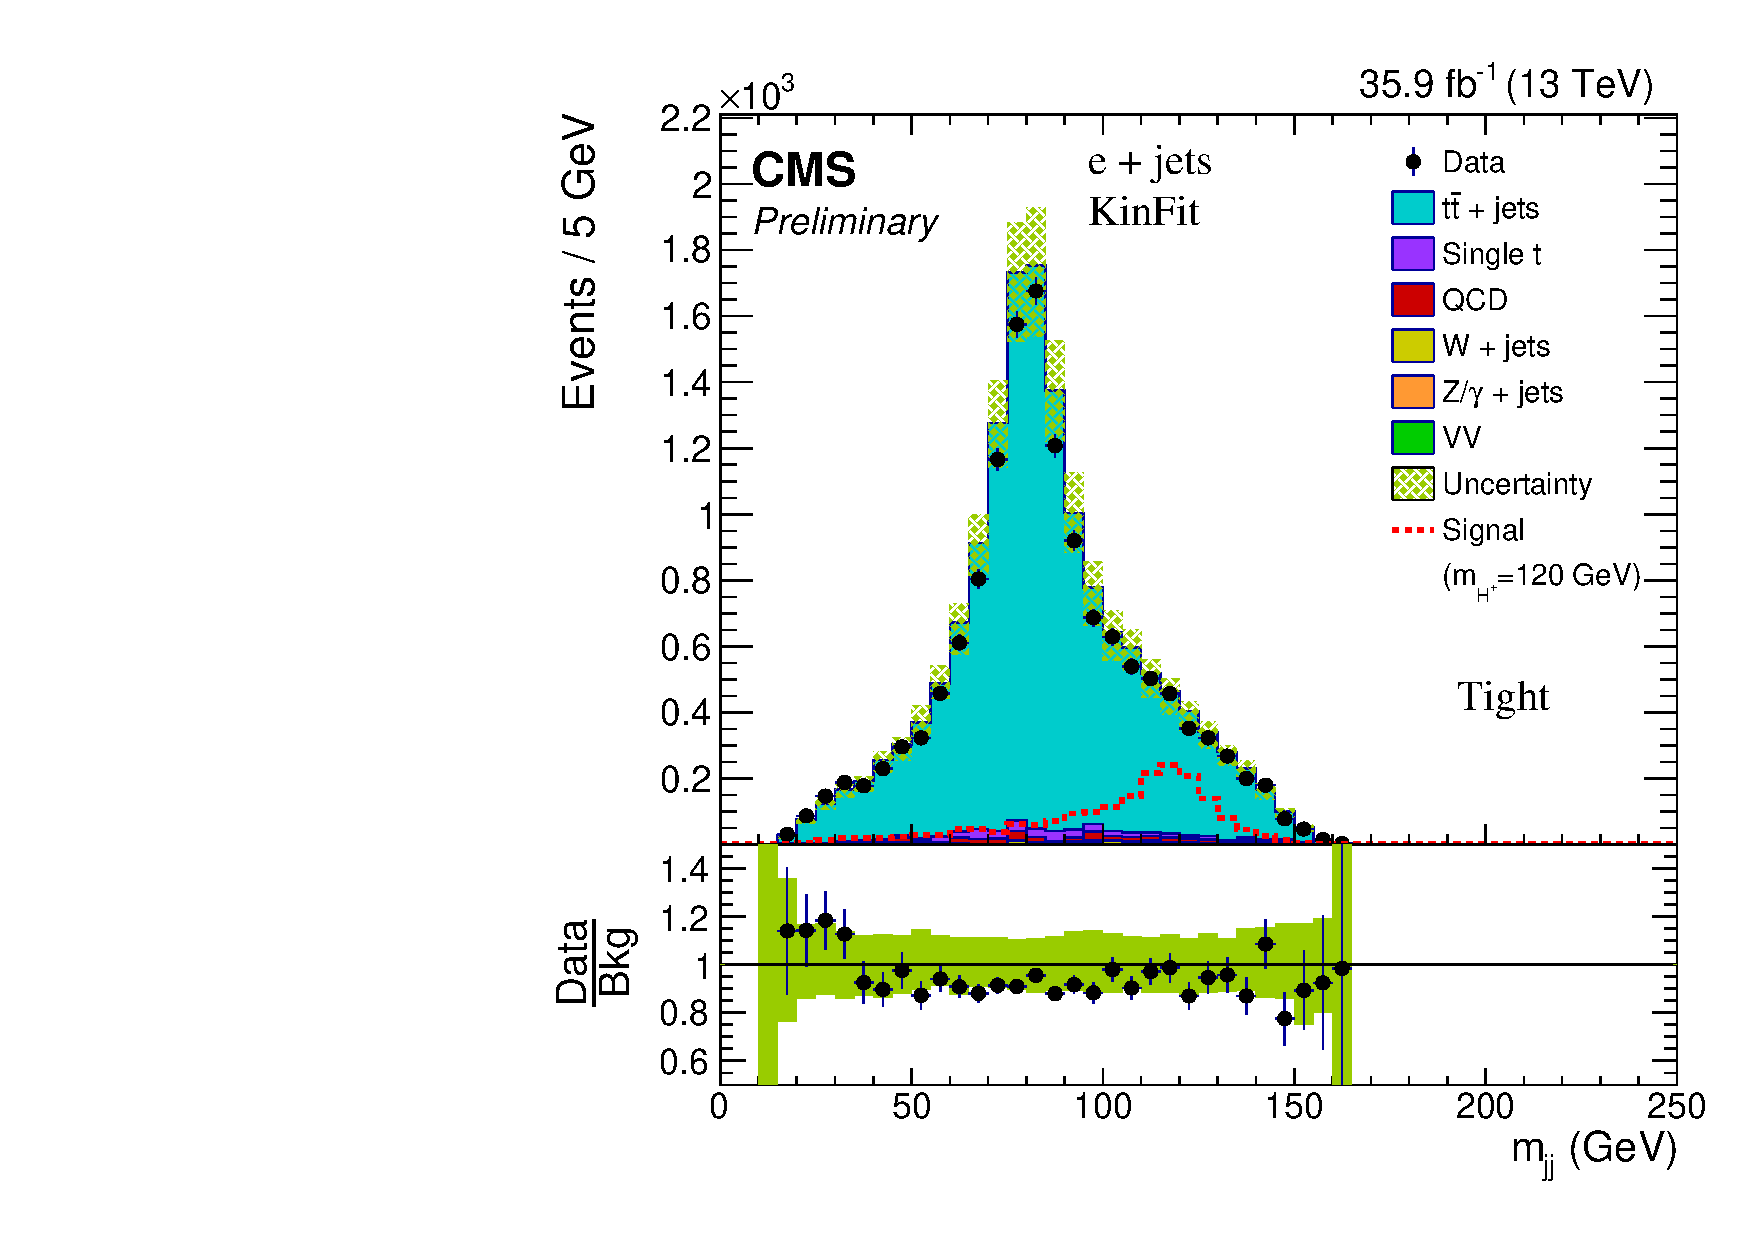
\includegraphics[width=0.44\textwidth]{Image/Appendix/mjj_kfit_CTagExT_eleKinFit.pdf}
\caption{Distribution of \mjj for the exclusive charm tagging 
    categories for the muon + jets (left column) and electron + jets 
    (right column) channel with statistical and systematic 
    uncertainties, prior to the fit to data. The upper row shows the 
    exclusive loose category, the middle row shows the exclusive 
    medium category, and the lower row shows the exclusive tight 
    category. The uncertainty band (upper absolute, lower relative)
    includes the statistical, as well as systematic components. The 
    signal events are scaled by twice the maximum observed upper limit on
    $\mathcal{B}(\PQt \to \PSHp\PQb)$ obtained at 
    8\TeV~\cite{Khachatryan:2015uua}.}
    \label{fig:mjjPreFit}
\end{figure}

\begin{figure}
\centering
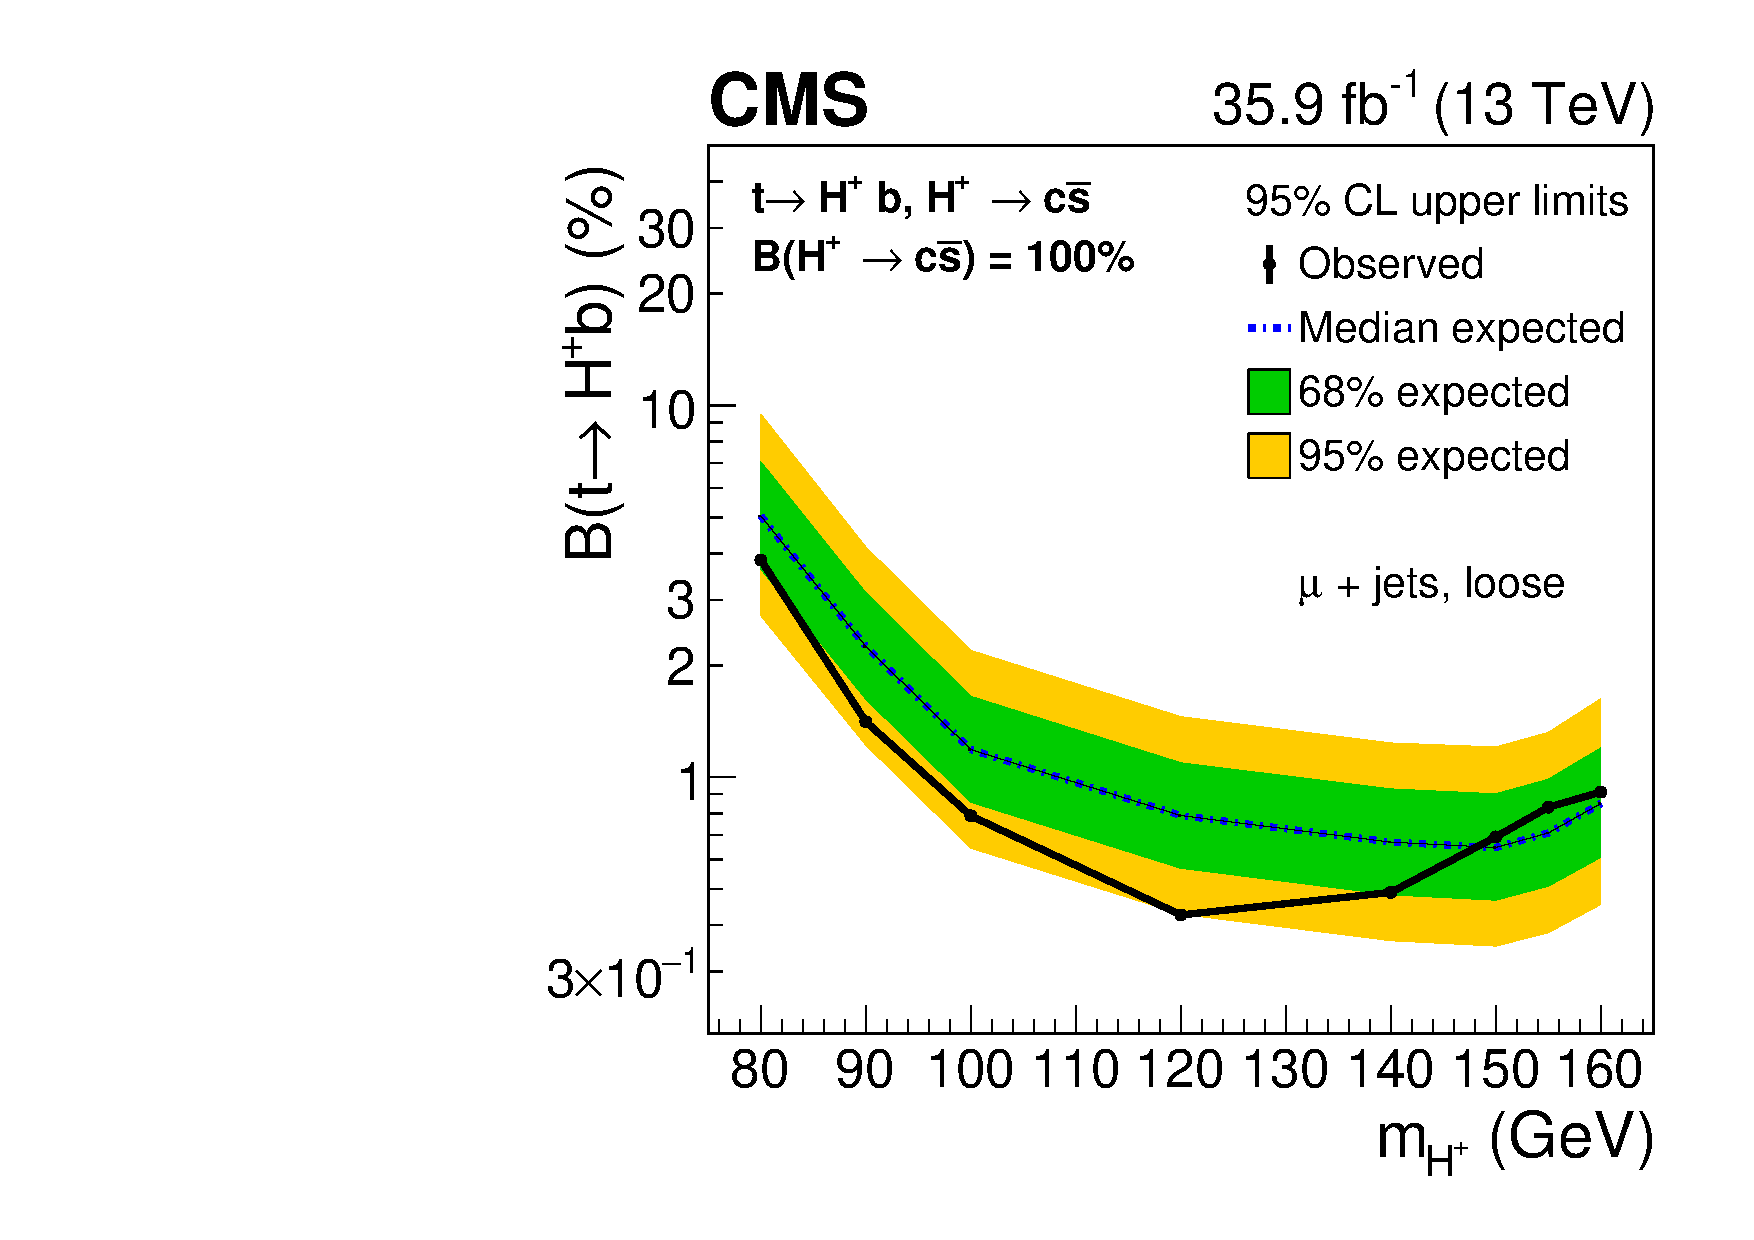
\includegraphics[width=0.45\textwidth]{Image/Appendix/limit_mu_ExL.pdf}
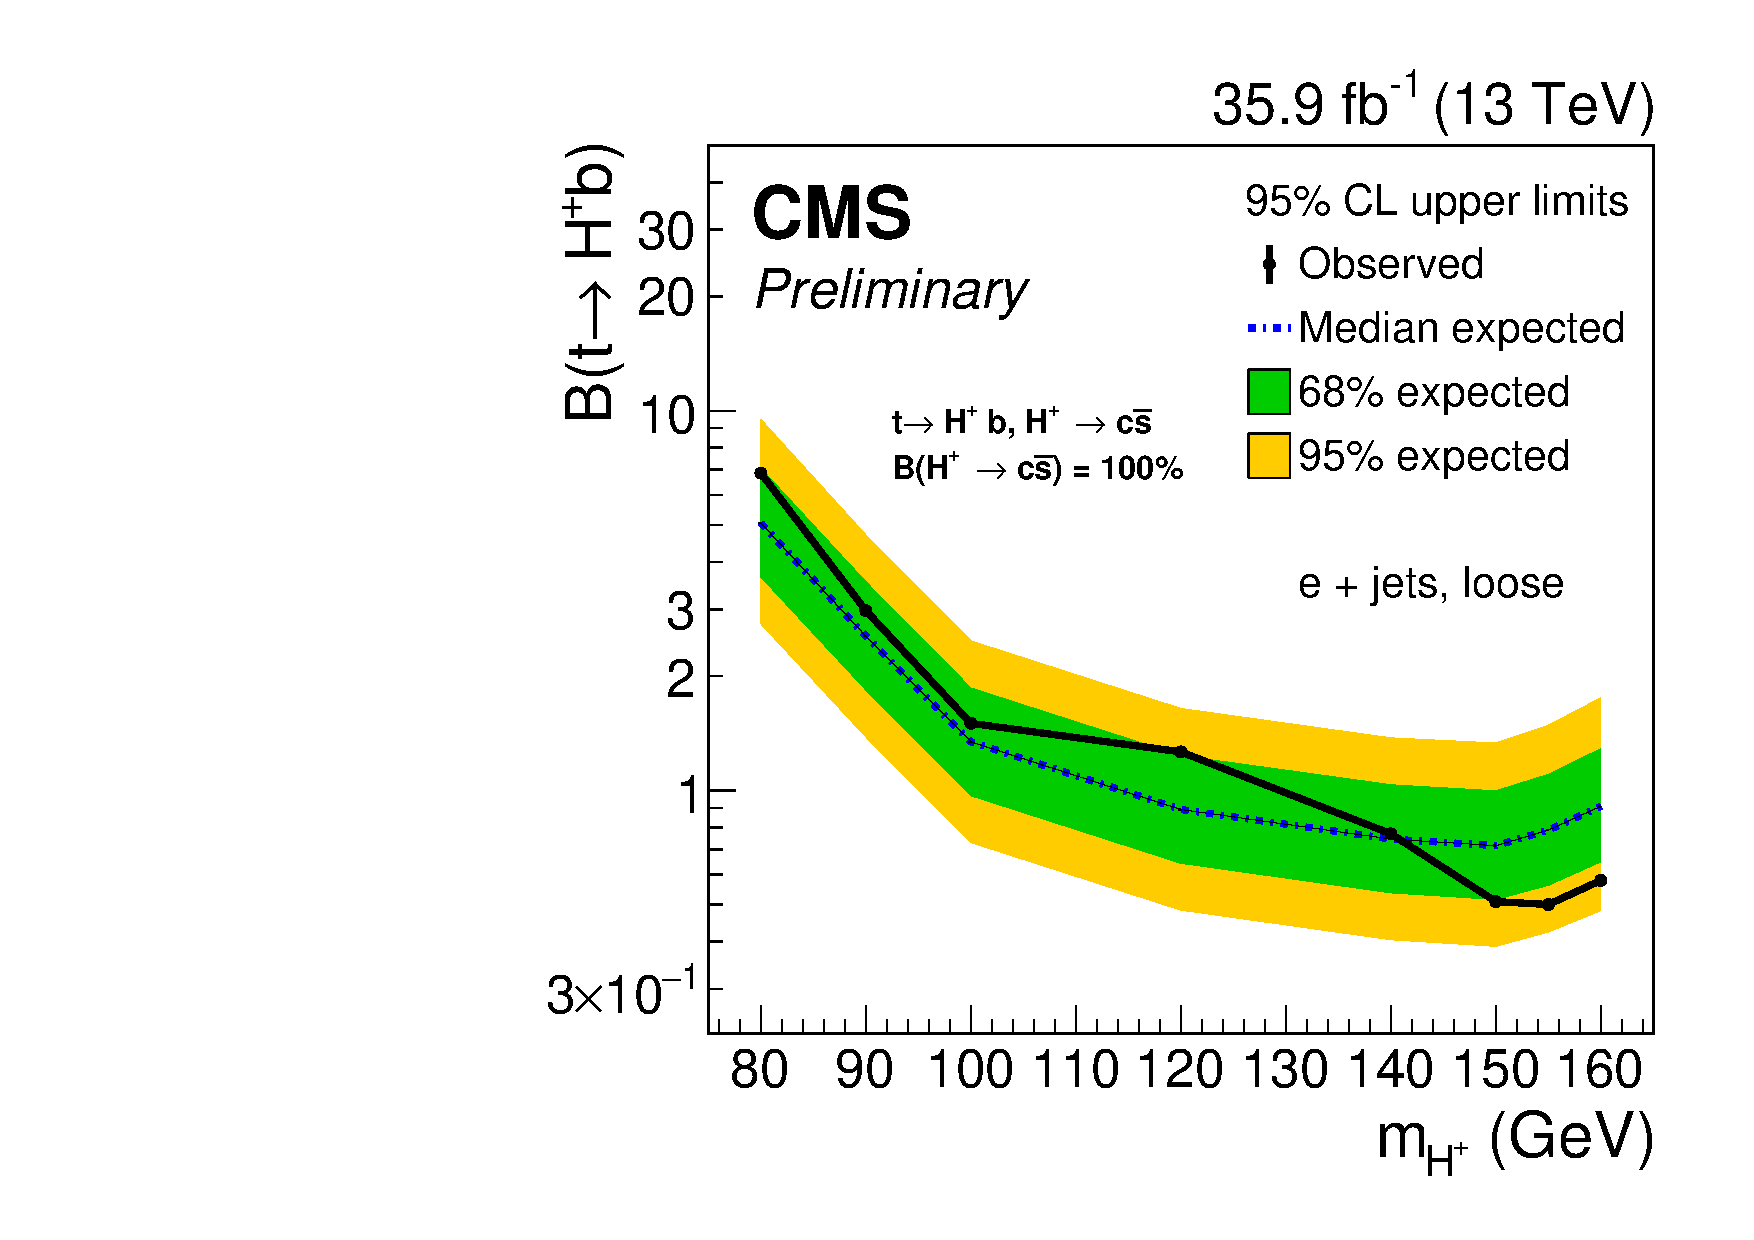
\includegraphics[width=0.45\textwidth]{Image/Appendix/limit_ele_ExL.pdf}
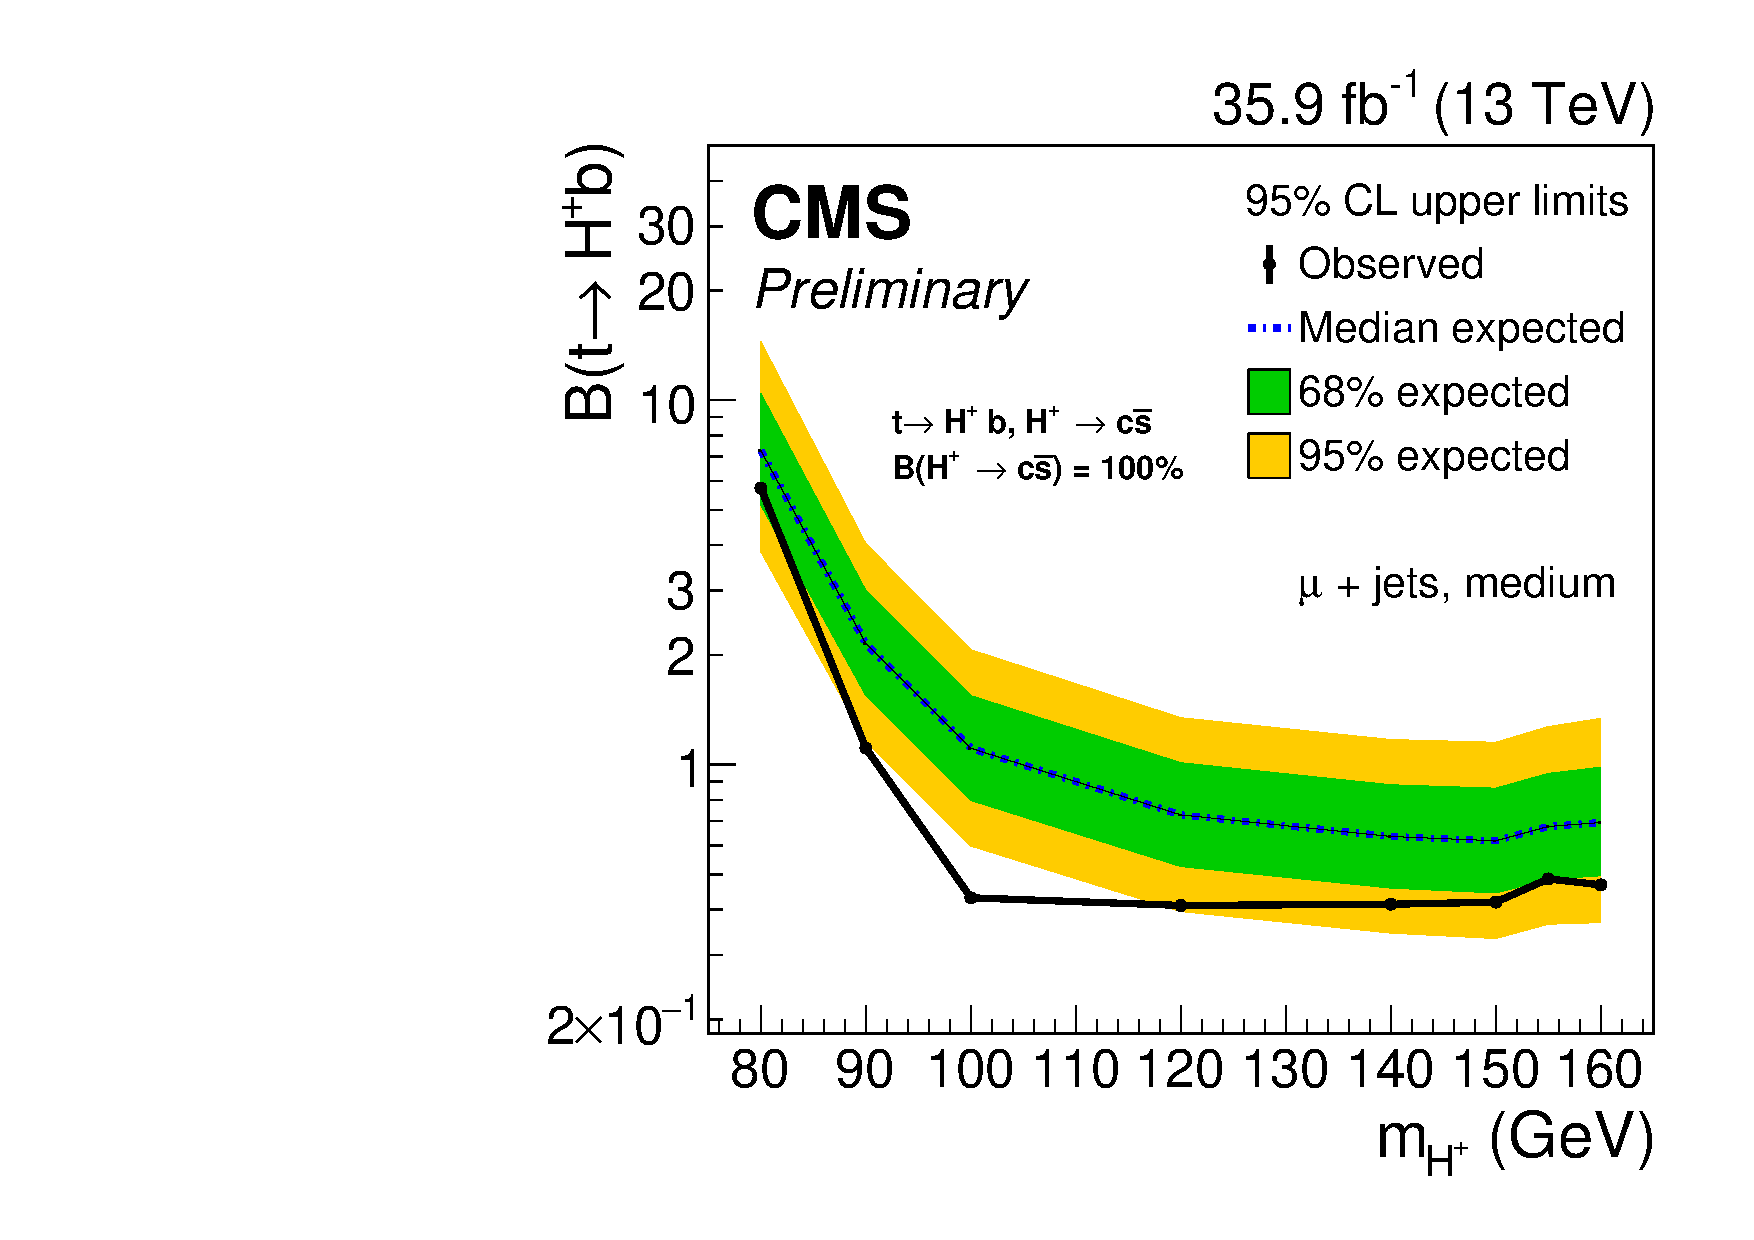
\includegraphics[width=0.45\textwidth]{Image/Appendix/limit_mu_ExM.pdf}
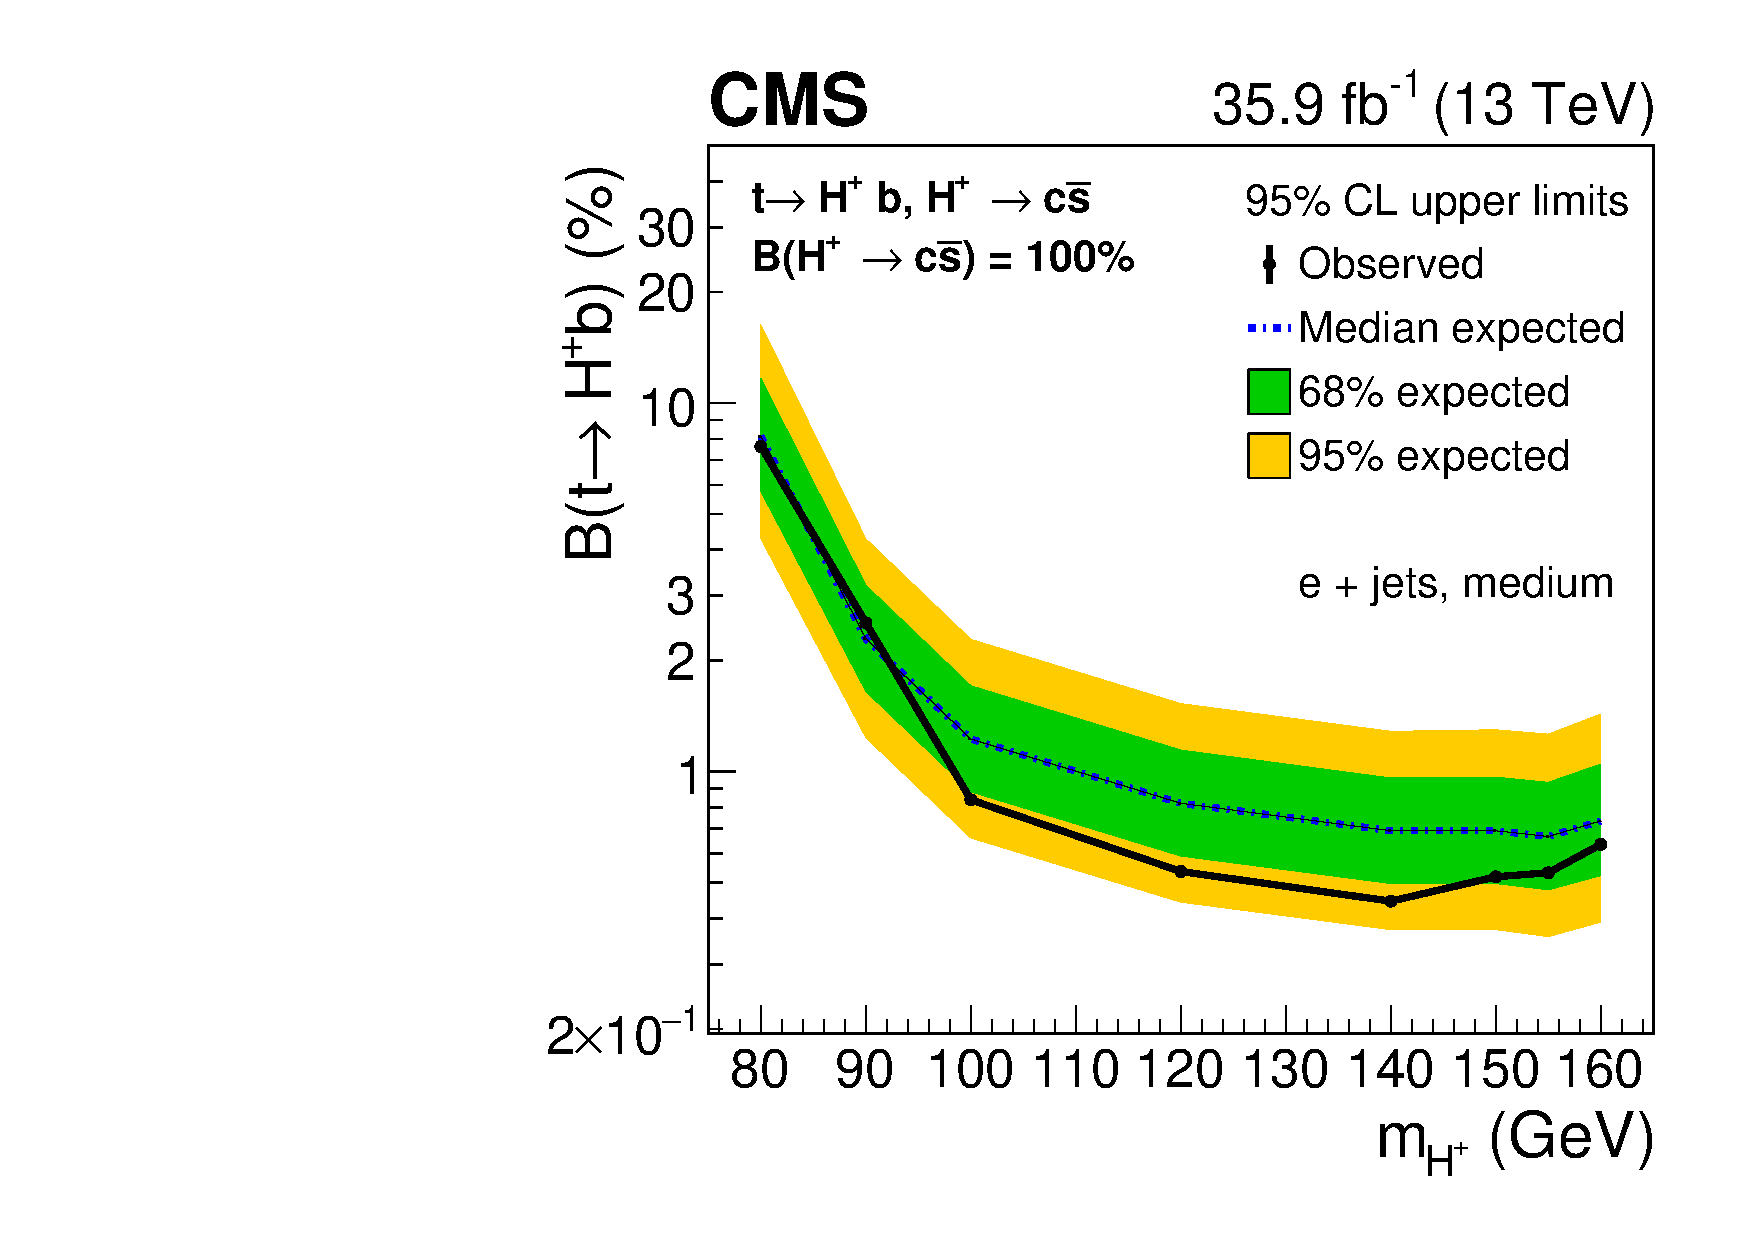
\includegraphics[width=0.45\textwidth]{Image/Appendix/limit_ele_ExM.pdf}
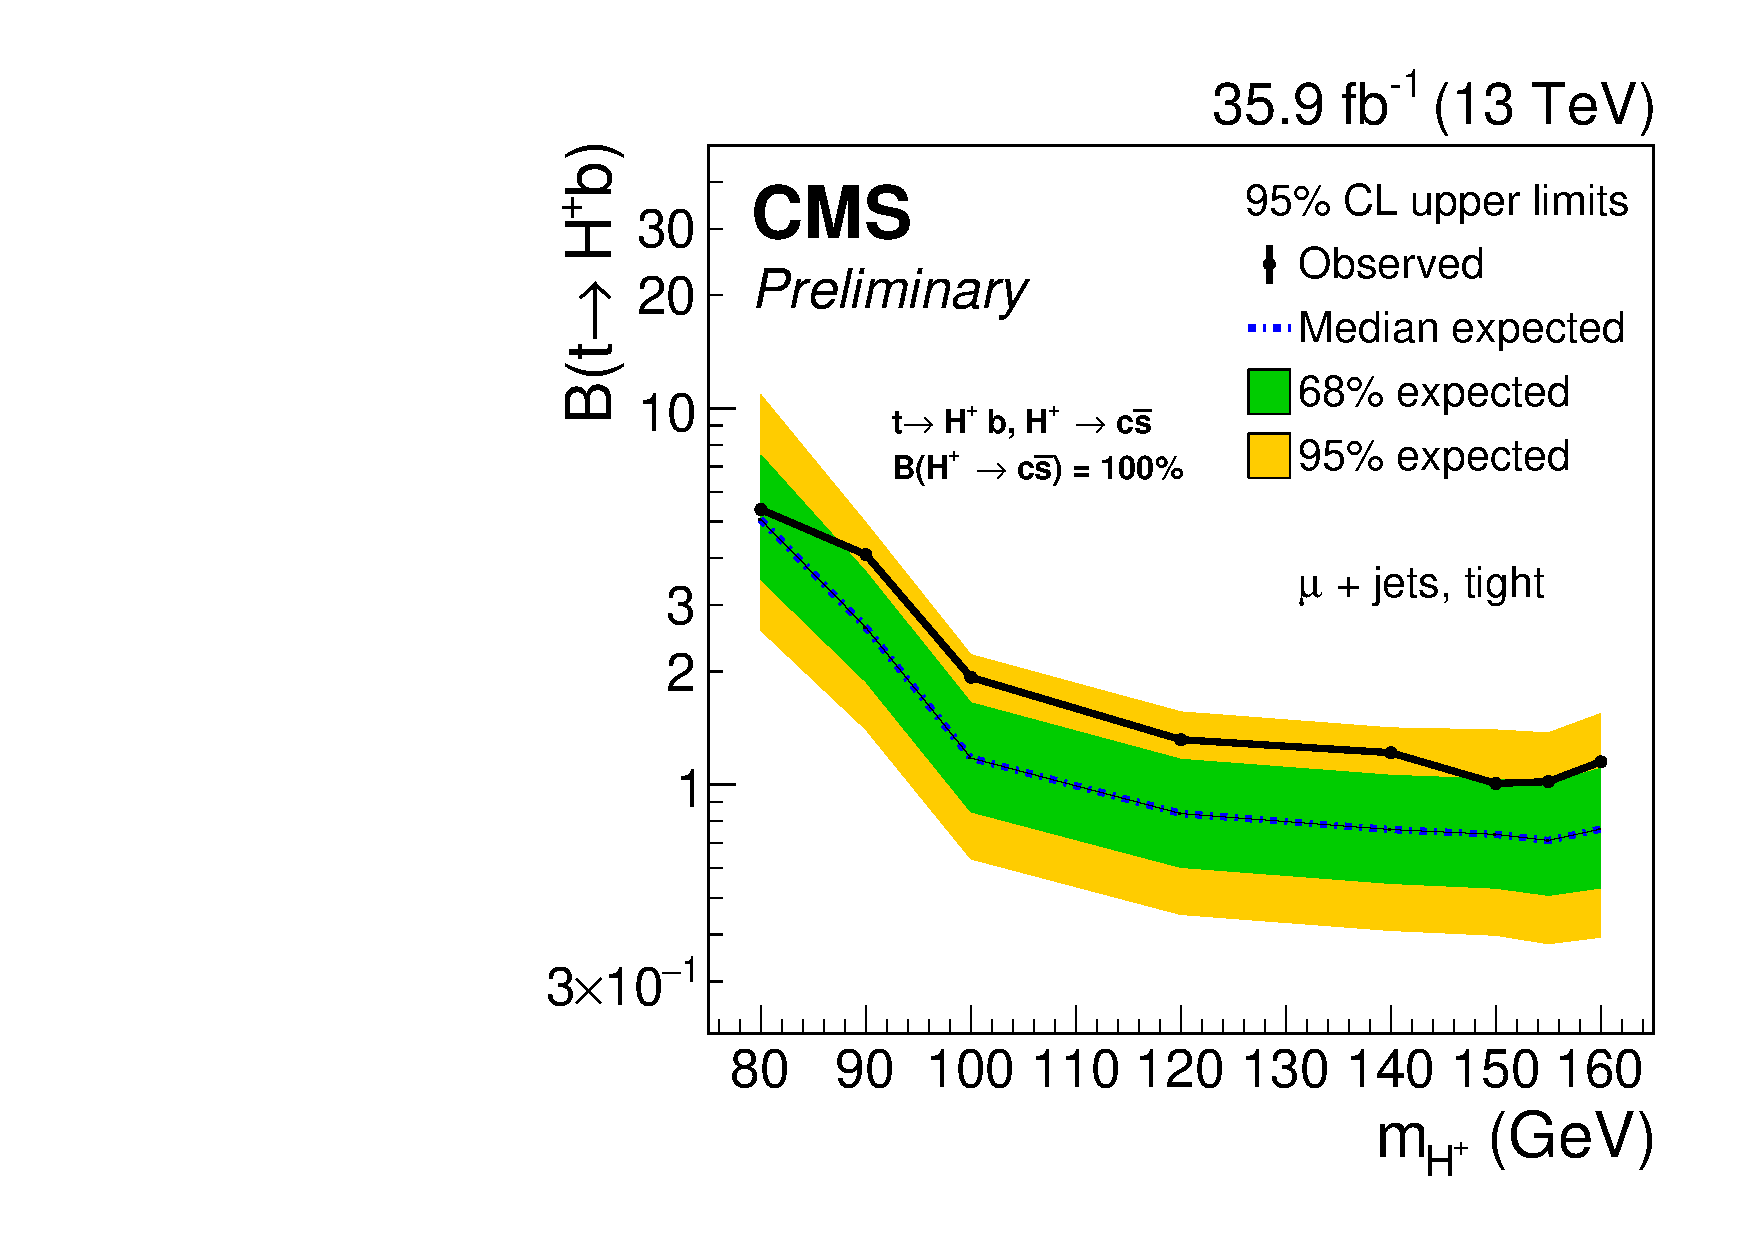
\includegraphics[width=0.45\textwidth]{Image/Appendix/limit_mu_ExT.pdf}
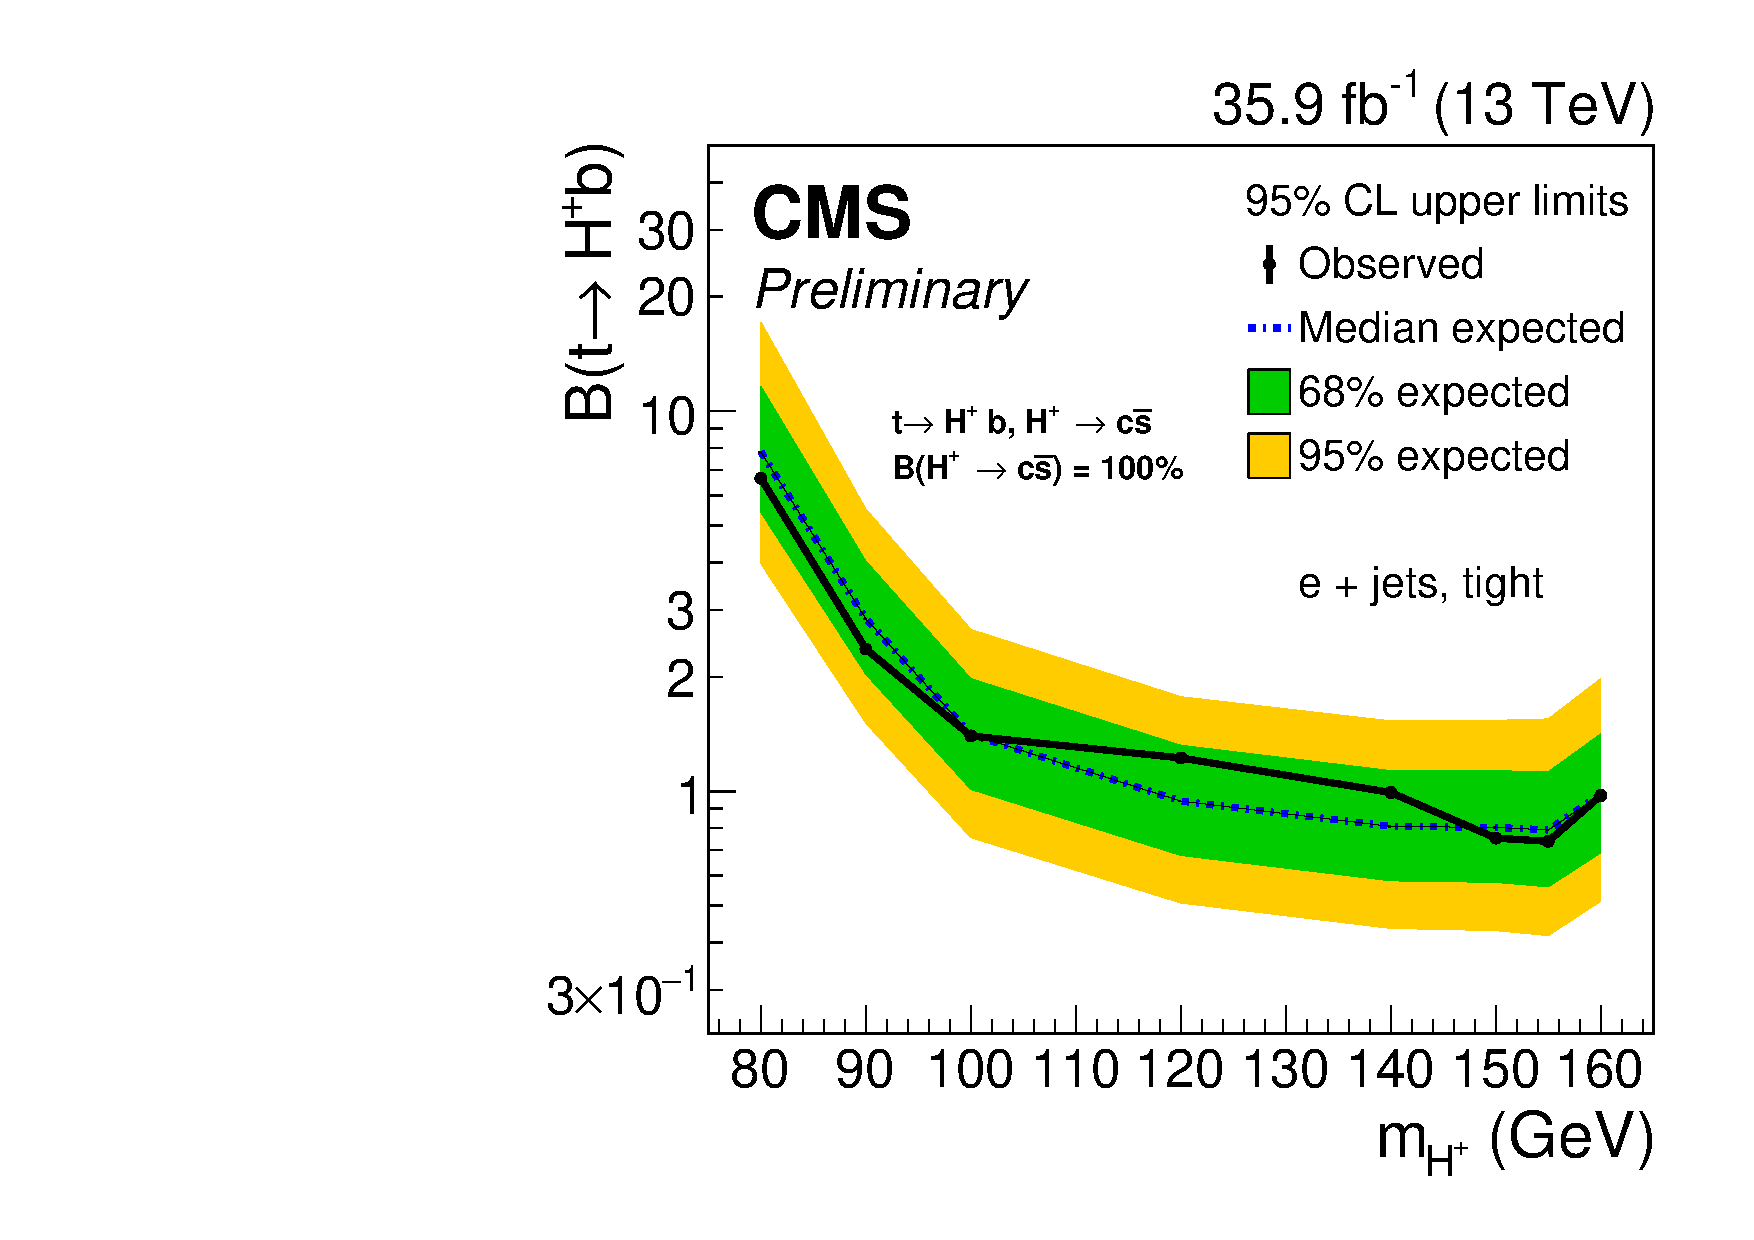
\includegraphics[width=0.45\textwidth]{Image/Appendix/limit_ele_ExT.pdf}
\caption{The expected and observed upper limit in \% on 
    $\mathcal{B} (\PQt \to \PSHp\PQb)$ as a function of $m_{\PSHp}$ 
    using \mjj for the different individual charm tagging categories 
    in the muon + jets (left column) and electron + jets (right column) 
    channel. The upper row shows the limits from the exclusive loose 
    category, the middle row the exclusive medium category, and the 
    lower row the exclusive tight category.}
    \label{fig:limitAppend}
\end{figure}

